\documentclass[a4paper,12pt]{article}
\usepackage[utf8]{inputenc}
\usepackage[T2A]{fontenc}
\usepackage[russian]{babel}
\usepackage{amsmath, amssymb}
\usepackage{graphicx}
\usepackage{geometry}
\geometry{top=2cm, bottom=2cm, left=2.5cm, right=1.5cm}
\usepackage{float}

\begin{document}

\begin{center}
    {\Large \textbf{Лабораторная работа №2.1.4}} \\
    \vspace{0.3cm}
    {\Large \textbf{Измерение теплоёмкости твёрдых тел}} \\
    \vspace{0.5cm}
    \textbf{Студент:} Михаил Орлов \\
    \textbf{Группа:} Б04-507 \\
    \textit{Дата выполнения:} 19 марта 2026 г.
\end{center}

\section*{Цель работы}
\begin{enumerate}
    \item Экспериментальное получение кривых разогрева $T_{\text{нагр}}(t)$ и остывания $T_{\text{охл}}(t)$ для пустого калориметра, а также для системы «калориметр + исследуемый образец».
    \item Вычисление коэффициента теплоотдачи стенок калориметра.
    \item Определение теплоёмкости пустого калориметра и удельной теплоёмкости исследуемых веществ.
\end{enumerate}

\section*{Оборудование}
В эксперименте использовались: калориметр со встроенным нагревателем и термометром сопротивления; мультиметр В7-78/3 в режиме омметра ($\sigma_T = 0.05$ К); термопара K-типа совместно с мультиметром В7-78/2 для измерения комнатной температуры ($\sigma_{T_{\text{комн}}} = 0.1$ К); источник питания GPS-72303; мультиметры В7-78/3 (режим амперметра, $\sigma_I = 0.01$ А) и KEITHLEY (режим вольтметра, $\sigma_U = 0.1$ В) для контроля мощности нагревателя; ПО АКИП для сбора данных с мультиметров ($\sigma_t = 0.01$ с).

\section{Теоретическое введение}
Теплоёмкость в данной работе рассчитывается по соотношению:
\begin{equation}
    C = \frac{\Delta Q}{\Delta T},
    \label{eq:def}
\end{equation}
где $\Delta Q$ — количество теплоты, сообщённое телу, $\Delta T$ — вызванное этим изменение температуры.

Измерение температуры внутри калориметра осуществляется с помощью термометра сопротивления. В реальных условиях не вся подводимая мощность идёт на нагрев системы, поскольку часть энергии теряется через стенки калориметра. С учётом теплопотерь:
\begin{equation}
    C\Delta T = P\Delta t - \lambda(T - T_k)\Delta T,
    \label{eq:base}
\end{equation}
где $\lambda$ — коэффициент теплоотдачи, $T$ — текущая температура калориметра, $T_k$ — температура окружающей среды.

В дифференциальной форме для режимов нагрева и остывания ($P=0$) уравнения имеют вид:
\begin{equation}
    \begin{aligned}
        C dT &= P dt - \lambda[T_{\text{нагр}}(t) - T_k(t)] dt, \\
        C dT &= -\lambda[T_{\text{охл}}(t) - T_k(t)] dt,
    \end{aligned}
    \label{eq:diff}
\end{equation}
где $P$ — мощность нагревателя, $t$ — время, отсчитываемое от момента включения нагревателя, $T_{\text{нагр}}(t)$ и $T_{\text{охл}}(t)$ — температуры на кривых нагрева и охлаждения соответственно, $T_k(t)$ — комнатная температура.

\subsection{Конструкция установки}
Калориметр помещён в пенопластовую изоляцию и размещён внутри ящика из многослойной фанеры. Внутренняя полость калориметра выполнена из материала с высокой теплопроводностью. Для обеспечения надёжного теплового контакта образцы и стенки имеют форму усечённых конусов, плотно сопрягающихся друг с другом.

В процессе эксперимента фиксируются:
\begin{enumerate}
    \item $R_{\text{нагр}}(t)$ — временная зависимость сопротивления термометра при нагреве калориметра с образцом при постоянной мощности.
    \item $R_{\text{охл}}(t)$ — временная зависимость сопротивления термометра при остывании калориметра с образцом (нагреватель отключён).
    \item $T_k(t)$ — изменение комнатной температуры во времени.
\end{enumerate}

\begin{figure}[H]
    \centering
    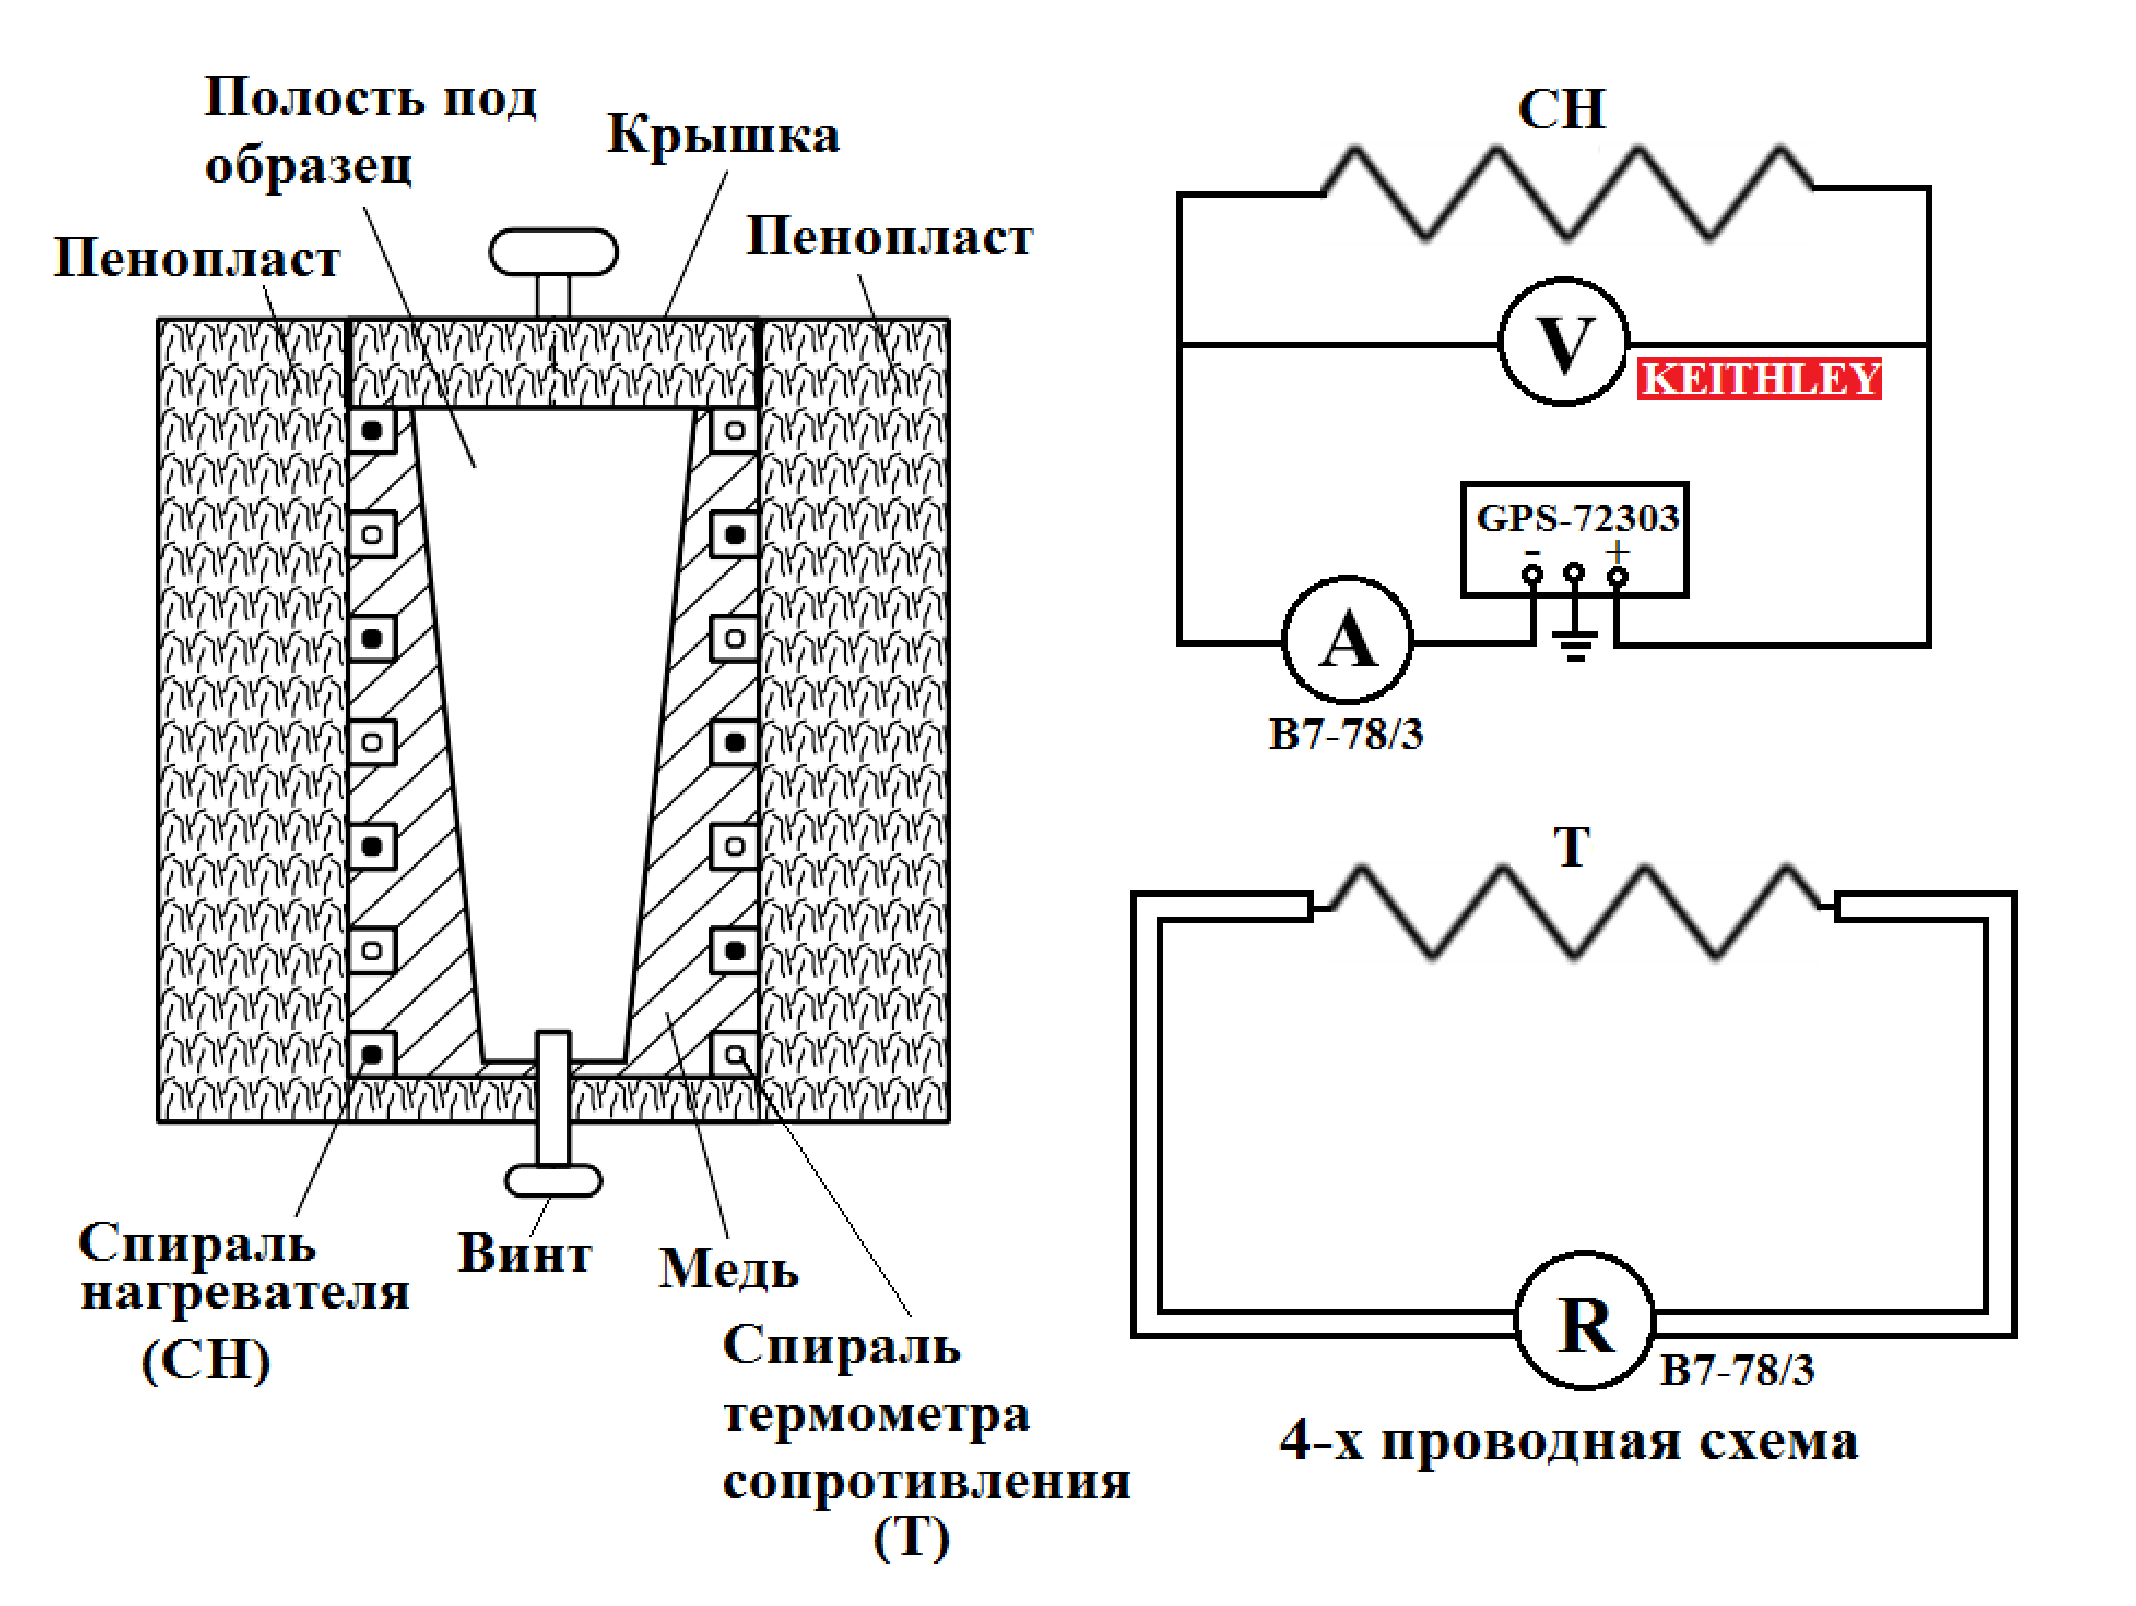
\includegraphics[width=0.6\textwidth]{schema_calorimeter.png}
    \caption{Принципиальная схема калориметра}
    \label{fig:schema}
\end{figure}

\subsection{Методика экспериментальных исследований}
Температура регистрируется с помощью термометра сопротивления, зависимость сопротивления от температуры описывается выражением:
\begin{equation}
    R_T = R_{273}(1 + \alpha(T - 273)),
    \label{eq:resistance}
\end{equation}
где $R_T$ — сопротивление при температуре $T$, $R_{273}$ — сопротивление при $0^\circ$C, $\alpha$ — температурный коэффициент.

Используя значение $R_k$ — сопротивление при комнатной температуре, находим:
\begin{equation}
    R_{273} = \frac{R_k}{1 + \alpha(T_k - 273)}.
    \label{eq:R273}
\end{equation}
Подстановка \eqref{eq:R273} в \eqref{eq:resistance} даёт:
\begin{equation}
    T(R_T) = 273 + \frac{R_T}{\alpha R_k} [1 + \alpha(T_k - 273)] - \frac{1}{\alpha}.
    \label{eq:T_from_R}
\end{equation}
Для меди $\alpha = 4.28 \times 10^{-3}$ K$^{-1}$.

При стационарной комнатной температуре ($T_k = \text{const}$) процесс остывания описывается уравнением:
\begin{equation}
    C dT_{\text{охл}} = -\lambda[T_{\text{охл}} - T_k] dt,
    \label{eq:cool_diff}
\end{equation}
интегрирование которого приводит к:
\begin{equation}
    T_{\text{охл}}(t) = (T_0 - T_k) e^{-\frac{\lambda}{C} t} + T_k.
    \label{eq:cool_exp}
\end{equation}
Соответственно, для нагрева:
\begin{equation}
    T_{\text{нагр}}(t) = \frac{P}{\lambda} \left(1 - e^{-\frac{\lambda}{C} t}\right) + T_k.
    \label{eq:heat_exp}
\end{equation}

\subsection{Дифференциальные методы обработки}
При заметных флуктуациях комнатной температуры предпочтительнее использовать дифференциальный подход. В момент, когда температура калориметра сравнивается с комнатной:
\begin{equation}
    C = \frac{P}{(dT_{\text{нагр}}/dt)_{T=T_k}}.
    \label{eq:diff_C}
\end{equation}

Другой способ основан на сопоставлении скоростей изменения температуры на кривых нагрева и остывания при одинаковой температуре $T$. Вводя обозначения $A = (dT/dt)_{\text{нагр}}$ и $B = (dT/dt)_{\text{охл}}$, получаем:
\begin{equation}
    \lambda = \frac{P}{(T - T_{k2})(1 - A/B) + T_{k2} - T_{k1}}, \quad
    C = \frac{P}{A - B + A \frac{T_{k1} - T_{k2}}{T - T_{k1}}}.
    \label{eq:diff_lambda_C}
\end{equation}
При $T_{k1} = T_{k2} = T_k$ формулы упрощаются:
\begin{equation}
    \lambda = \frac{P}{(T - T_k)(1 - A/B)}, \quad
    C = \frac{P}{A - B}.
    \label{eq:diff_simple}
\end{equation}

\section{Экспериментальная часть}

\subsection{Временная разметка эксперимента}
Согласно записям в лабораторном журнале:
\begin{itemize}
    \item 10:40 — начало повышения температуры после предварительного охлаждения.
    \item 10:46 — запуск нагревателя (пустой калориметр).
    \item 11:06 — отключение нагревателя.
    \item 11:20 — начало остывания.
    \item 11:26 — возобновление роста температуры.
    \item 11:31 — включение нагревателя с образцом алюминия.
    \item 11:50 — выключение нагревателя.
    \item 12:08 — начало остывания.
    \item 12:18 — включение нагревателя с образцом железа.
    \item 12:25 — выключение нагревателя.
\end{itemize}

\subsection{Процедура измерений}

\subsubsection{Предварительное охлаждение калориметра}
В калориметр устанавливается охлаждённый конус. Через 4 минуты после начала устойчивого роста температуры конус извлекается, и система выдерживается ещё 4 минуты. Калориметр оказывается охлаждённым примерно на 5 $^\circ$C ниже комнатной температуры.

\subsubsection{Нагрев пустого калориметра}
Включается нагреватель. После достижения перегрева относительно комнатной температуры на 9 $^\circ$C питание нагревателя отключается.

\subsubsection{Охлаждение пустого калориметра}
Регистрация температуры продолжается. После снижения температуры на 2 $^\circ$C от максимального значения приступают к измерениям с образцом.

\subsubsection{Повторное охлаждение}
Калориметр вновь охлаждается на 5 $^\circ$C ниже комнатной температуры, после чего в него помещается исследуемый образец, и циклы нагрева-охлаждения повторяются.

\subsubsection{Исследуемые материалы}
Для измерений использовались образцы алюминия и железа:
\begin{equation}
    m_{\text{Al}} = (294.1 \pm 0.5) \text{ г}, \qquad m_{\text{Fe}} = (814.8 \pm 0.5) \text{ г}.
\end{equation}

\subsubsection{Завершение}
Запись данных останавливается, файлы с результатами сохраняются.

\section{Обработка экспериментальных данных}

\subsection{Идентификация временных интервалов}
Общий вид полученных зависимостей приведён на рис. \ref{fig:full}. Соответствие временных отрезков различным этапам эксперимента представлено в таблице \ref{tab:times}.

\begin{table}[H]
    \centering
    \begin{tabular}{|l|c|c|}
        \hline
        \textbf{Процесс} & \textbf{Начало, с} & \textbf{Окончание, с} \\
        \hline
        $T_{\text{нагр1}}(t)$ — нагрев пустого калориметра & 1000 & 2500 \\
        $T_{\text{охл1}}(t)$ — охлаждение пустого калориметра & 2600 & 3700 \\
        $T_{\text{нагр2}}(t)$ — нагрев с алюминием & 4800 & 6000 \\
        $T_{\text{охл2}}(t)$ — охлаждение с алюминием & 6300 & 6900 \\
        $T_{\text{нагр3}}(t)$ — нагрев с железом & 7800 & 8600 \\
        $T_{\text{охл3}}(t)$ — охлаждение с железом & 8800 & 9300 \\
        \hline
    \end{tabular}
    \caption{Привязка кривых к временным интервалам}
    \label{tab:times}
\end{table}

Вариации комнатной температуры в ходе опыта не превышали 2 К, что обосновывает применимость интегрального метода расчёта.

\subsection{Дифференциальный метод для пустого калориметра}
Сначала определим теплоёмкость пустого калориметра с использованием дифференциальных соотношений.

По формуле \eqref{eq:diff_C} в окрестности точки пересечения кривой нагрева с уровнем комнатной температуры (при $dT = 0.5$ К):
\begin{equation}
    C_{\text{кал}} = (0.68 \pm 0.16) \ \frac{\text{кДж}}{\text{К}}.
\end{equation}

Используя \eqref{eq:diff_simple} для температуры $T = 304.5$ К:
\begin{equation}
    C_{\text{кал}} = (0.72 \pm 0.17) \ \frac{\text{кДж}}{\text{К}}.
\end{equation}

В качестве итогового значения примем среднее:
\begin{equation}
    C_{\text{кал}} = (0.70 \pm 0.12) \ \frac{\text{кДж}}{\text{К}}.
\end{equation}

\subsection{Дифференциальный метод для алюминия}
Для образца алюминия по формуле \eqref{eq:diff_C}:
\begin{equation}
    C_{\text{Al}} = (0.21 \pm 0.18) \ \frac{\text{кДж}}{\text{К}}, \qquad
    c_{\text{Al}} = (0.71 \pm 0.61) \ \frac{\text{кДж}}{\text{кг} \cdot \text{К}}.
\end{equation}

По формуле \eqref{eq:diff_simple}:
\begin{equation}
    C_{\text{Al}} = (0.19 \pm 0.17) \ \frac{\text{кДж}}{\text{К}}, \qquad
    c_{\text{Al}} = (0.65 \pm 0.58) \ \frac{\text{кДж}}{\text{кг} \cdot \text{К}}.
\end{equation}

\subsection{Дифференциальный метод для железа}
Для железного образца по формуле \eqref{eq:diff_C}:
\begin{equation}
    C_{\text{Fe}} = (0.33 \pm 0.20) \ \frac{\text{кДж}}{\text{К}}, \qquad
    c_{\text{Fe}} = (0.41 \pm 0.25) \ \frac{\text{кДж}}{\text{кг} \cdot \text{К}}.
\end{equation}

По формуле \eqref{eq:diff_simple}:
\begin{equation}
    C_{\text{Fe}} = (0.31 \pm 0.19) \ \frac{\text{кДж}}{\text{К}}, \qquad
    c_{\text{Fe}} = (0.38 \pm 0.23) \ \frac{\text{кДж}}{\text{кг} \cdot \text{К}}.
\end{equation}

\subsection{Интегральный метод для пустого калориметра}
Для пустого калориметра построена полулогарифмическая анаморфоза кривой охлаждения (рис. \ref{fig:cool_empty}). После исключения начального нелинейного участка методом наименьших квадратов определён угловой коэффициент, который в соответствии с \eqref{eq:cool_exp} равен $-\lambda/C$.

\begin{figure}[H]
    \centering
    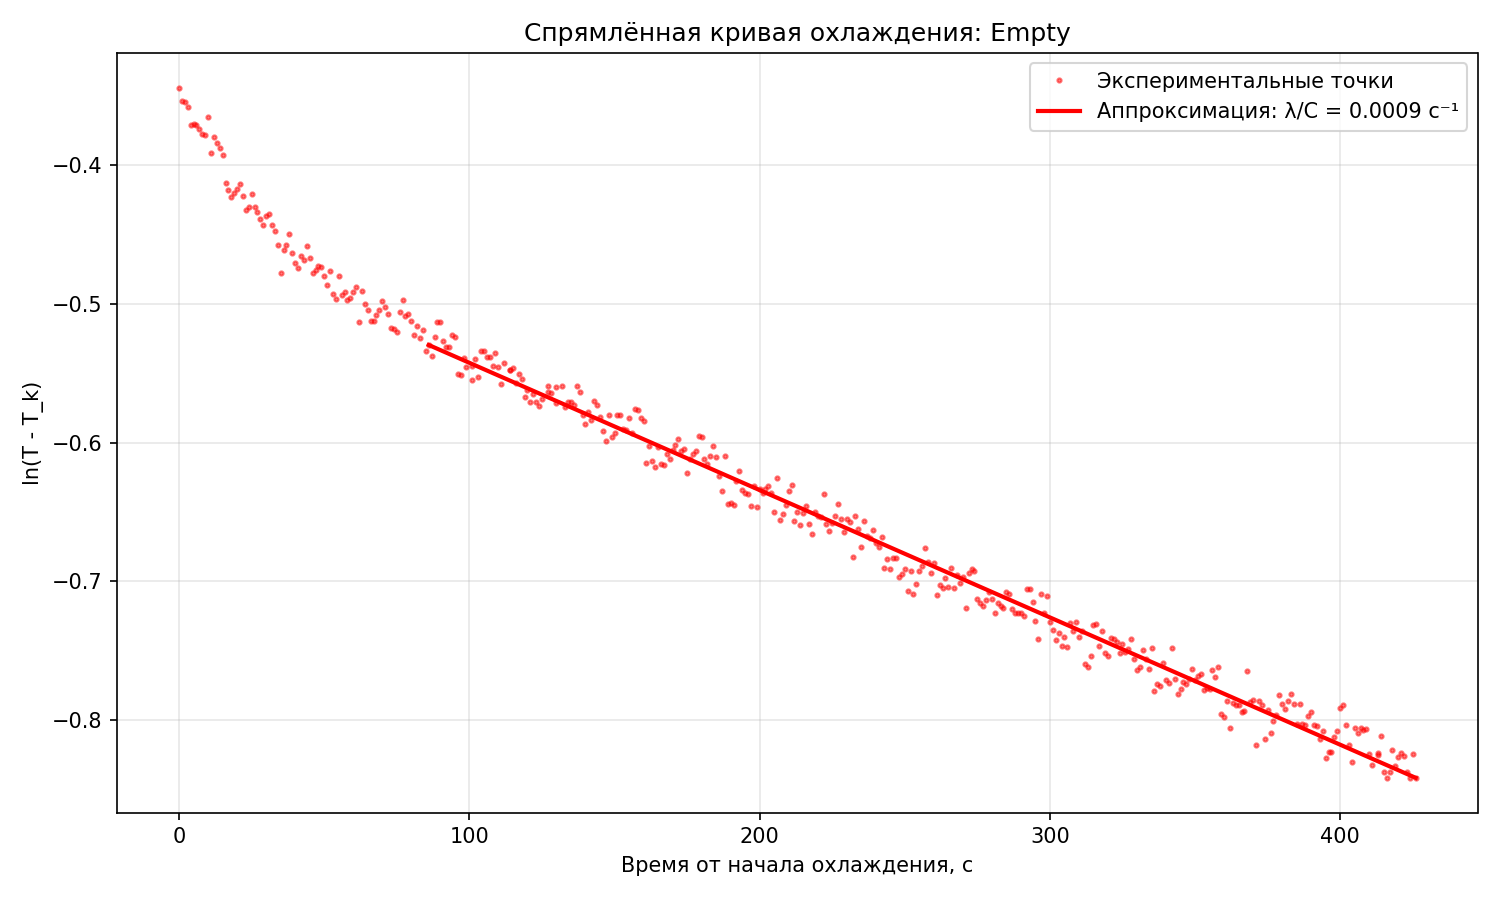
\includegraphics[width=0.7\textwidth]{cooling_empty.png}
    \caption{Полулогарифмический график охлаждения пустого калориметра}
    \label{fig:cool_empty}
\end{figure}

Полученное отношение:
\begin{equation}
    \frac{\lambda}{C_{\text{кал}}} = (34 \pm 2) \times 10^{-5} \text{ c}^{-1}.
\end{equation}

Аппроксимация кривой нагрева по \eqref{eq:heat_exp} даёт значение $\lambda$:
\begin{equation}
    \lambda = (0.25 \pm 0.02) \ \frac{\text{Вт}}{\text{К} \cdot \text{с}}.
\end{equation}
Теплоёмкость пустого калориметра:
\begin{equation}
    C_{\text{кал}} = \lambda \Big/ \frac{\lambda}{C_{\text{кал}}} = (0.74 \pm 0.06) \ \frac{\text{кДж}}{\text{К}}.
\end{equation}

\subsection{Интегральный метод для алюминия}
Аналогичная обработка для системы с алюминиевым образцом (рис. \ref{fig:cool_al}) даёт:

\begin{figure}[H]
    \centering
    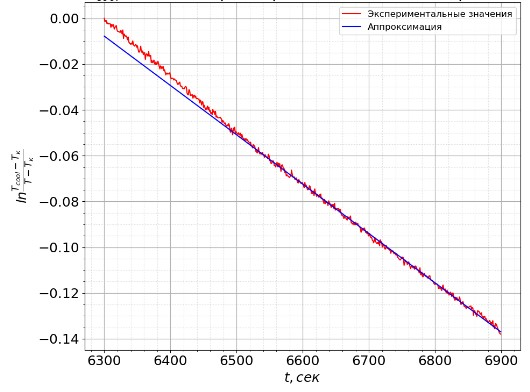
\includegraphics[width=0.7\textwidth]{cooling_aluminum}
    \caption{Полулогарифмический график охлаждения калориметра с алюминием}
    \label{fig:cool_al}
\end{figure}

\begin{equation}
    \frac{\lambda}{C_{\text{сум,Al}}} = (21 \pm 3) \times 10^{-5} \text{ c}^{-1}, \qquad
    \lambda = (0.22 \pm 0.03) \ \frac{\text{Вт}}{\text{К} \cdot \text{с}}.
\end{equation}
Суммарная теплоёмкость:
\begin{equation}
    C_{\text{сум,Al}} = \lambda \Big/ \frac{\lambda}{C_{\text{сум,Al}}} = (1.05 \pm 0.16) \ \frac{\text{кДж}}{\text{К}}.
\end{equation}
Теплоёмкость образца:
\begin{equation}
    C_{\text{Al}} = C_{\text{сум,Al}} - C_{\text{кал}} = (0.31 \pm 0.17) \ \frac{\text{кДж}}{\text{К}}.
\end{equation}
Удельная теплоёмкость:
\begin{equation}
    c_{\text{Al}} = \frac{C_{\text{Al}}}{m_{\text{Al}}} = (1.05 \pm 0.58) \ \frac{\text{кДж}}{\text{кг} \cdot \text{К}}.
\end{equation}

\subsection{Интегральный метод для железа}
Для системы с железным образцом (рис. \ref{fig:cool_fe}):

\begin{figure}[H]
    \centering
    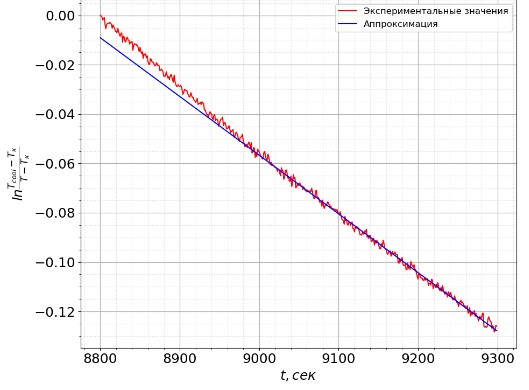
\includegraphics[width=0.7\textwidth]{cooling_iron}
    \caption{Полулогарифмический график охлаждения калориметра с железом}
    \label{fig:cool_fe}
\end{figure}

\begin{equation}
    \frac{\lambda}{C_{\text{сум,Fe}}} = (18 \pm 3) \times 10^{-5} \text{ c}^{-1}, \qquad
    \lambda = (0.21 \pm 0.03) \ \frac{\text{Вт}}{\text{К} \cdot \text{с}}.
\end{equation}
Суммарная теплоёмкость:
\begin{equation}
    C_{\text{сум,Fe}} = \lambda \Big/ \frac{\lambda}{C_{\text{сум,Fe}}} = (1.17 \pm 0.19) \ \frac{\text{кДж}}{\text{К}}.
\end{equation}
Теплоёмкость образца:
\begin{equation}
    C_{\text{Fe}} = C_{\text{сум,Fe}} - C_{\text{кал}} = (0.43 \pm 0.20) \ \frac{\text{кДж}}{\text{К}}.
\end{equation}
Удельная теплоёмкость:
\begin{equation}
    c_{\text{Fe}} = \frac{C_{\text{Fe}}}{m_{\text{Fe}}} = (0.53 \pm 0.25) \ \frac{\text{кДж}}{\text{кг} \cdot \text{К}}.
\end{equation}

\section{Обсуждение результатов}
Справочные значения удельной теплоёмкости:
\begin{equation}
    c_{\text{Al}}^{\text{табл}} = 0.902 \ \frac{\text{кДж}}{\text{кг} \cdot \text{К}}, \qquad
    c_{\text{Fe}}^{\text{табл}} = 0.450 \ \frac{\text{кДж}}{\text{кг} \cdot \text{К}}.
\end{equation}

Полученные в работе результаты сведены в таблицу \ref{tab:results}.

\begin{table}[H]
    \centering
    \begin{tabular}{|l|c|c|c|}
        \hline
        \textbf{Материал} & \textbf{Метод} & $\mathbf{c}$, кДж/(кг·К) & $\mathbf{C}$, кДж/К \\
        \hline
        Алюминий & интегральный & $1.05 \pm 0.58$ & $0.31 \pm 0.17$ \\
        Алюминий & дифференциальный & $0.68 \pm 0.60$ & $0.20 \pm 0.18$ \\
        Железо & интегральный & $0.53 \pm 0.25$ & $0.43 \pm 0.20$ \\
        Железо & дифференциальный & $0.40 \pm 0.24$ & $0.32 \pm 0.20$ \\
        \hline
    \end{tabular}
    \caption{Сравнение результатов, полученных разными методами}
    \label{tab:results}
\end{table}

Все измеренные значения в пределах погрешностей согласуются с табличными данными. Для алюминия интегральный метод даёт несколько завышенное значение, что может быть связано с неточным определением начального участка кривой охлаждения. Для железа, напротив, интегральный метод даёт результат ближе к табличному, чем дифференциальный.

Погрешности дифференциального метода выше, поскольку для вычисления производной используется малый участок кривой, что увеличивает влияние случайных погрешностей измерения температуры. Различия в результатах, полученных разными методами, находятся в пределах заявленных погрешностей, что свидетельствует о корректности проведённых измерений.

\section{Заключение}
В ходе лабораторной работы:
\begin{itemize}
    \item Зарегистрированы кривые нагревания и охлаждения пустого калориметра, а также систем с образцами алюминия и железа.
    \item Определён коэффициент теплоотдачи стенок калориметра $\lambda = 0.23 \pm 0.03$ Вт/(К·с).
    \item Вычислена теплоёмкость пустого калориметра $C_{\text{кал}} = 0.72 \pm 0.09$ кДж/К.
    \item Получены значения удельной теплоёмкости алюминия и железа, согласующиеся с табличными в пределах погрешностей измерений.
\end{itemize}

\section{Приложение}

\begin{figure}[H]
    \centering
    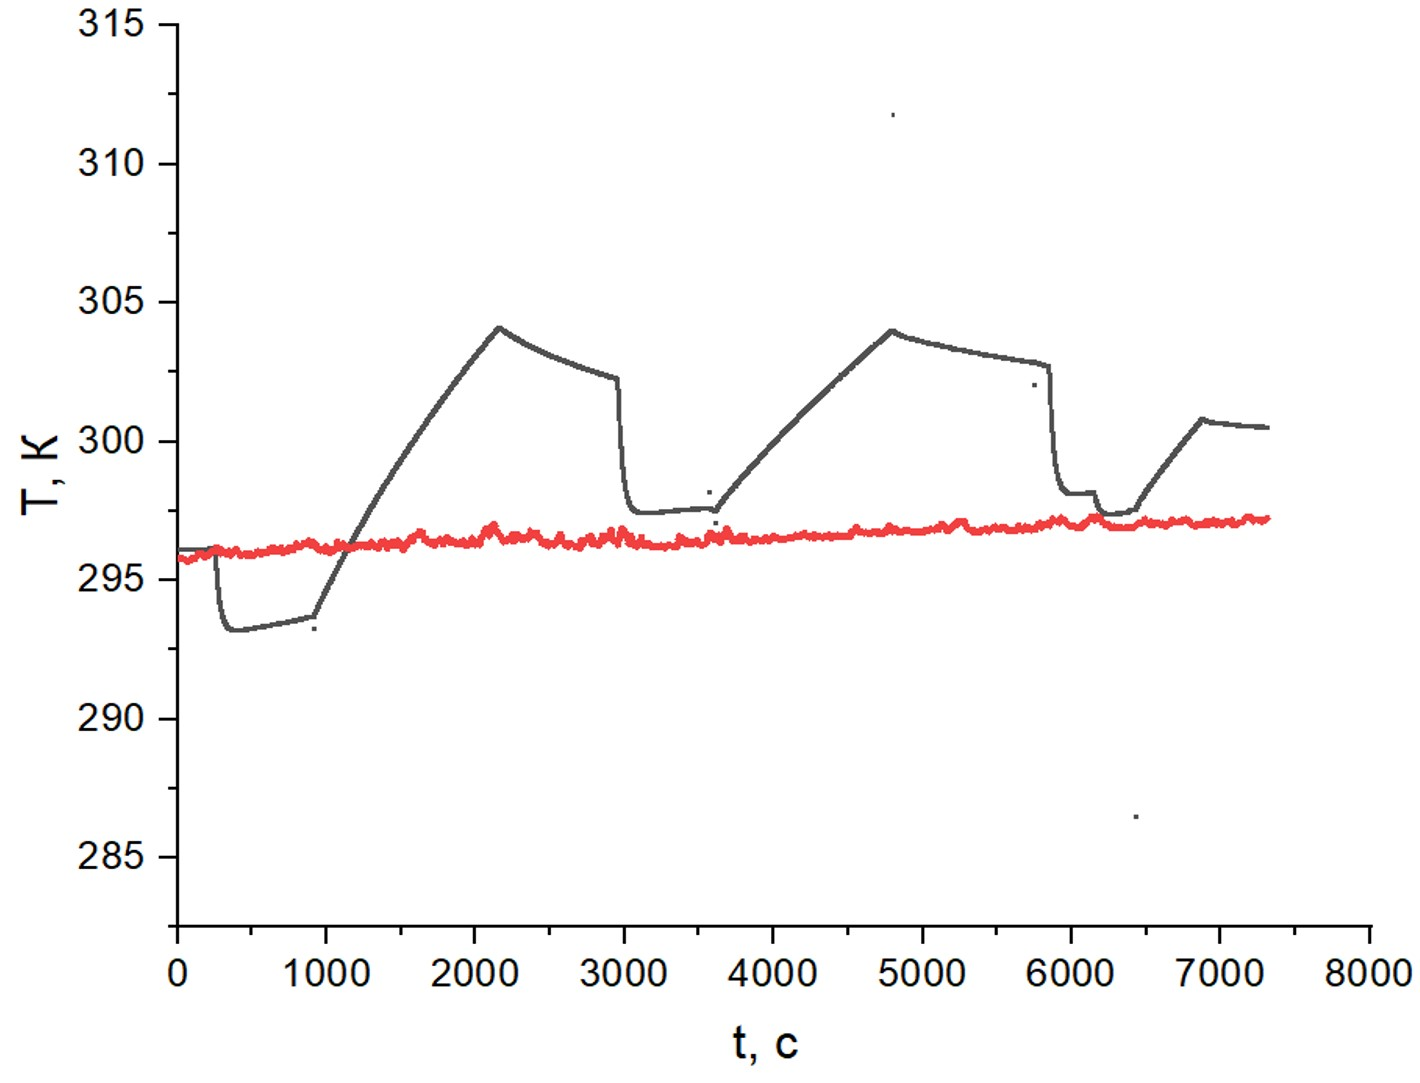
\includegraphics[width=0.9\textwidth]{full_experiment}
    \caption{Полный временной ход температур калориметра и окружающей среды}
    \label{fig:full}
\end{figure}

\end{document}